\documentclass{article}
\usepackage{../../typesetting/styles/report-zh}

% Set document information
\title{周报~向嘉豪 (\today)}
\author{向嘉豪}
\date{\today}

\begin{document}

\maketitle

\begin{abstract}
  本周我主要完成了三项工作:首先,完成了SLH-DSA算法在签名生成、公钥创建和验证过程中的自适应线程分配实验,结果显示我们的优化方案实现了显著性能提升,最高达到20\%;其次,对论文进行了全面的语言风格优化,使文本更符合学术写作规范;最后,完成了实验章节的详细框架设计,并基于学长建议提出了``基本操作并行效率"(POPE)这一新的评估指标。
\end{abstract}

\begin{weekplan}
1) 完成POPE指标实验验证,进一步量化分析不同安全级别下的资源利用效率
2) 准备完整的实验数据与可视化图表,提升论文的说服力
\end{weekplan}

\section{论文实验}

本周我们完成了对SLH-DSA算法在签名生成、公钥创建和验证过程中的自适应线程分配实验。如图~\ref{fig:expriment}所示,与\cite{Wang2025}的基准实现相比,我们的优化方案在各个阶段均实现了显著的性能提升,其中签名生成阶段的性能增益最为显著,达到了\textcolor{blue}{20\%}的提升。

实验数据表明,在资源密集型操作(如签名生成过程中的哈希计算)中,优化效果尤为明显。这与我们的理论分析一致,即通过精确识别算法瓶颈并实施针对性优化,可以显著提升整体执行效率。

\begin{figure}[htbp]
\centering
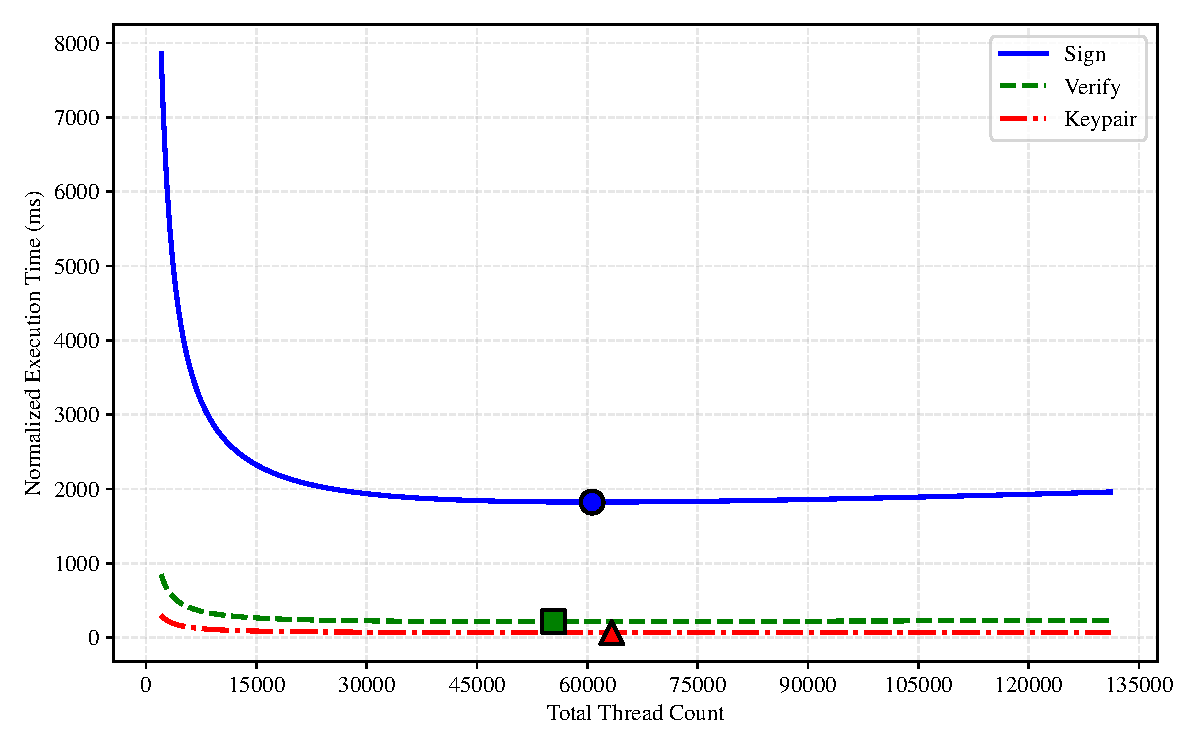
\includegraphics[width=0.5\textwidth]{./fig/thread_efficiency.pdf}
\caption{自适应线程分配实验结果}
\label{fig:expriment}
\end{figure}

\section{论文写作}

\subsection{口语表达修正}

为提升论文的学术严谨性,我们对全文进行了系统性的语言风格调整。具体修订包括:(1) 将一般性描述替换为具有学科特定意义的专业术语;(2) 优化句法结构,消除冗余表达,增强论述精确度;(3) 重构段落组织,确保论证逻辑连贯且层次分明;(4) 统一采用学术写作中的规范化被动语态;(5) 精炼图表说明文字,提高信息传递效率。

如图~\ref{fig:example}所示,我们将``is"替换为更具描述性的``represents",将``main"替换为``fundamental"等, 通过这些系统性修改,论文的语言表达更加符合高水平计算密码学研究领域的表达惯例与标准。

\begin{figure}[htbp]
\centering
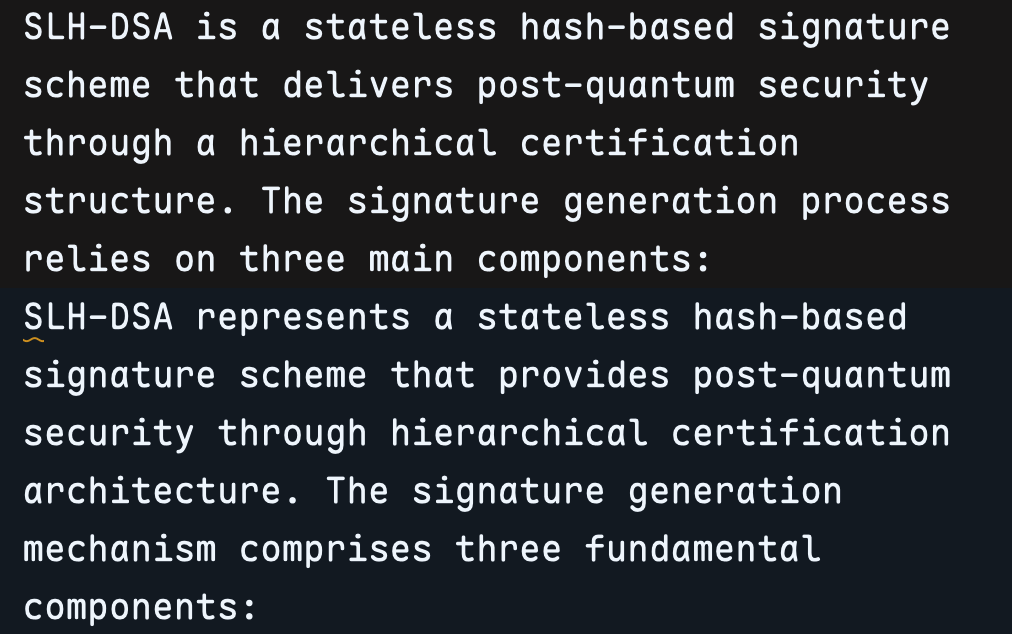
\includegraphics[width=0.5\textwidth]{./fig/fix_writing.png}
\caption{学术语言风格优化示例}
\label{fig:example}
\end{figure}

\subsection{实验章节写作}
本周完成了论文实验章节的详细框架设计,该章节旨在通过严谨的实验方法评估SLH-DSA算法优化实现的性能。实验体系由五个相互关联的部分构成:

实验体系整合了五个相互关联的核心方面:基于NVIDIA RTX 4090 GPU的硬件平台配置与NIST标准参数集的实验环境设置;通过精确测量各组件执行时间定量评估ATA算法对密码学核心函数的优化贡献;与传统串行实现对比评估FLP技术在不同安全级别下的加速效果;将我们的实现与NIST参考代码和最新GPU实现进行执行时间、吞吐量和资源利用率等多维度对比;以及在不同安全参数下测试性能变化趋势并引入能耗效率指标(性能/瓦特)评估优化方案的实际应用价值。全面的实验设计确保了研究结果的科学性和可靠性,为我们的优化方法提供了坚实的实证支持。

\subsection{新叙述角度POPE}

根据学长的指导,我们探索了一种新颖的评估角度,以更全面地阐述我们的优化贡献。传统上,签名算法优化往往侧重于整体执行时间的缩短,而忽略了底层计算资源利用效率的提升机制。我们提出将``基本操作并行效率"(Primitive Operation Parallel Efficiency, POPE)作为评估指标,专门度量在密码学算法不可进一步分解的基本操作P上的线程利用率。

POPE指标的核心优势在于:首先,它直接反映了并行架构中最小计算单元的利用效率,避免了传统指标可能掩盖的低层次资源浪费;其次,它建立了密码学算法特性与并行计算资源分配策略之间的直接联系,为算法设计者提供明确的优化方向;最后,它能够预测不同安全参数下算法性能的可扩展性,提供更具前瞻性的性能评估视角。

我们计划在下一阶段工作中,将POPE指标应用于实验分析,通过量化不同安全级别下的POPE变化趋势,验证我们的优化方法在资源利用方面的优越性。

% Replace standard bibliography commands with conditional version
\printbibliographyifcited[alpha]{../../paper}

\end{document}
